\usetikzlibrary{calc}
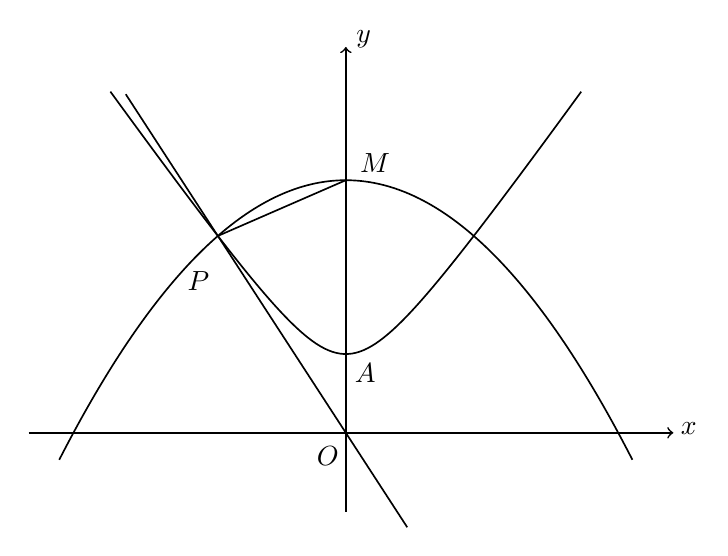
\begin{tikzpicture}[x=.65cm,y=1cm,line width=0.6pt,color=black,font=\normalsize]
% Axes
\draw[->] (-6.2,0)--(6.4,0);
\draw[->] (0,-1.0)--(0,4.9);
% y=-x line (through P and origin), extended both ways
\draw[solid] (-4.3,4.3)--(1.2,-1.2);
% Parabola: vertex M(0,3.20773797371), focus A(0,1)... schematic with m=3.207,a=2.5:
% x^2=-4(m-1)(y-m), y = m - x^2/(4(m-1))
\draw[solid,domain=-5.6:5.6,samples=160] plot (\x,{3.20773797371-\x*\x/(4*(3.20773797371-1))});
% Hyperbola upper branch: y=sqrt(1+0.84 x^2)
\draw[solid,domain=-4.6:4.6,samples=120] plot (\x,{sqrt(1+0.84*\x*\x)});
% Segment P-M
\draw[solid] (-2.5,2.5)--(0,3.20773797371);
% Key points
\coordinate (O) at (0,0);
\coordinate (Apt) at (0,1.0);
\coordinate (Mpt) at (0,3.20773797371);
\coordinate (Ppt) at (-2.5,2.5);
% labels with clearance
\node[inner sep=1pt] at (6.7,0.05) {$x$};
\node[inner sep=1pt] at (0.35,5.0) {$y$};
\node[inner sep=1pt] at (-0.35,-0.30) {$O$};
\node[below right=2pt,inner sep=1pt] at (Apt) {$A$};
\node[right=2pt,inner sep=1pt] at (0.1,3.42) {$M$};
\node[below left=2pt,inner sep=1pt,xshift=2.00bp,yshift=-4.00bp] at (-2.6,2.3) {$P$};
\end{tikzpicture}
